%
% Descripción del cifrador BC de BPS, presentación de cifrados que preservan 
% el formato.
% Proyecto Lovelace.
%

\subsection{Cifrador Interno BC}

%------------------------------------------------------------------------------
\begin{frame}{BPS}{Cifrador interno $BC$}

  Este cifrador se define como:
    \begin{equation}
      BC_{F,s,b,w}(X,K,T)
    \end{equation}
    
  Donde:
  \begin{itemize}
    \item $F$ es un cifrador por bloques de $f$ bits de salida.
    \item $s$ es la cardinalidad del conjunto de caracteres $S$.
    \item $b$ es la longitud del bloque. ($b \leq 2 \cdot |log_s(2^{f-32})|$)
    \item $w$ es el número de rondas de la red Feistel interna. (par)
    \item $X$ es la cadena de longitud $b$ a cifrar.
    \item $K$ es una llave acorde a $F$.
    \item $T$ es un tweak de 64 bits.
  \end{itemize}
  
\end{frame}

%------------------------------------------------------------------------------
\begin{frame}{BPS}{Cifrador interno $BC$}

  El cifrador $BC$ sigue el siguiente proceso para cifrar un bloque.
  
  \begin{enumerate}  
    \item Dividir el tweak $T$ en 2 subtweaks $T_L$ y $T_R$ de 32 bits.
      \begin{align}
        T_R\: &=\: T\: \mod\: 2^{32}  \\
        T_L\: &=\: (T\: -\: T_R) / 2^{32}
      \end{align}
  \end{enumerate}
  
\end{frame}

%------------------------------------------------------------------------------
\begin{frame}{BPS}{Cifrador interno $BC$}

  \begin{enumerate}
    \setcounter{enumi}{1}
    \item Dividir la cadena $X$ en 2 para obtener $X_L$ y $X_R$ con 
      longitudes $l$ y $r$ respectivamente. 
      
      Si $b$ es par: 
      \begin{equation}
        l =\: r\: =\: b/2
      \end{equation}

      Si $b$ es impar:
      \begin{align}
        l &=\: (b+1)/2 \\
        r &=\: (b-1)/2
      \end{align}
  \end{enumerate}
  
\end{frame}

%------------------------------------------------------------------------------
\begin{frame}{BPS}{Cifrador interno $BC$}

  \begin{enumerate}
    \setcounter{enumi}{2}
    \item Definir e inicializar $L_0$ y $R_0$.
      \begin{align}
        L_0\: &=\: \sum_{j=0}^{l-1} X_L[j] \cdot s^j \\
        R_0\: &=\: \sum_{j=0}^{r-1} X_R[j] \cdot s^j
      \end{align}    
  \end{enumerate}
  
\end{frame}

%------------------------------------------------------------------------------
\begin{frame}{BPS}{Cifrador interno $BC$}

  \begin{enumerate}
    \setcounter{enumi}{3}
    \item Partiendo de $i\: =\: 1$ hasta $i\: <\: w$:

      Si $i$ es par:
      \begin{align}
        L_{i+1}\: &=\: L_i\: \boxplus\: 
                      F_K((T_R \oplus i) \cdot 2^{f-32}\: +\: R_i)\quad 
                      (mod\ s^l) \\
        R_{i+1}\: &=\: R_i
      \end{align}
  
      Si $i$ es impar:
      \begin{align}
        R_{i+1}\: &=\: R_i\: \boxplus\: 
                      F_K((T_L \oplus i) \cdot 2^{f-32}\: +\: L_i)\quad 
                      (mod\ s^r) \\
        L_{i+1}\: &=\: L_i
      \end{align}
  \end{enumerate}
  
\end{frame}

%------------------------------------------------------------------------------
\begin{frame}{BPS}{Cifrador interno $BC$}

  \begin{enumerate}
    \setcounter{enumi}{4}
    \item Descomponer $L_w$ y $R_w$ para obtener a $Y_L$ y a $Y_R$, las 
      cuales concatenadas ($Y_L \parallel Y_R$) dan la cadena de salida $Y$.
  \end{enumerate}

    \begin{figure}[H]
      \begin{center}
        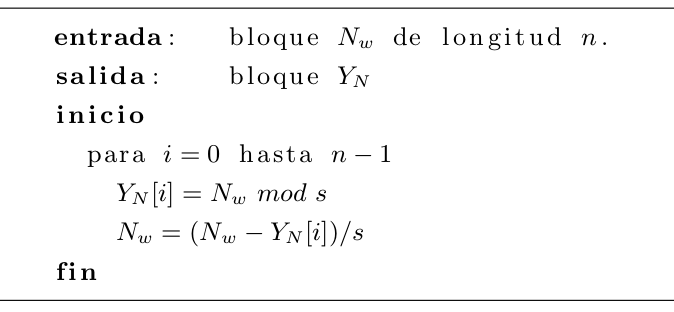
\includegraphics[width=0.75\linewidth]{diagramas/descomposicion}
        \caption{Proceso para descomponer $L_w$ y $R_w$.}
       \end{center}
    \end{figure}


\end{frame}

%------------------------------------------------------------------------------
\begin{frame}{BPS}{Descifrador $BC^{-1}$}

  Ahora, el proceso para descifrar la cadena $Y$ es:

  \begin{enumerate}
    \item Dividir $Y$ para obtener las subcadenas $Y_L$ y $Y_R$ con una 
      longitud $l$ y $r$ respectivamente, de igual forma que se hizo con 
      la cadena $X$ en el proceso de cifrado.    

    \item Definir e inicializar $L_w$ y $R_w$ en:
      \begin{align}
        L_w\: &=\: \sum_{j=0}^{l-1} Y_L[j] \cdot s^j \\
        R_w\: &=\: \sum_{j=0}^{r-1} Y_R[j] \cdot s^j
      \end{align}
  \end{enumerate}
\end{frame}

%------------------------------------------------------------------------------
\begin{frame}{BPS}{Descifrador $BC^{-1}$}

  \begin{enumerate}
    \setcounter{enumi}{2}
    \item Comenzando con $i=w-1$, para cada ronda $i\: \geq\: 0$.

    Si $i$ es par:
    \begin{align}
      L_i\: &=\: L_{i+1}\: \boxminus\: 
                E_K((T_R \oplus i) \cdot 2^{f-32}\: +\: R_{i+1})\quad 
                (mod\ s^l) \\
      R_i\: &=\: R_{i+1}
    \end{align}

    Si $i$ es impar:
    \begin{align}
      R_i\: &=\: R_{i+1}\: \boxminus\: 
                E_K((T_L \oplus i) \cdot 2^{f-32}\: +\: L_{i+1})\quad 
                (mod\ s^r) \\
      L_i\: &=\: L_{i+1}
    \end{align}

  \end{enumerate}
\end{frame}

%------------------------------------------------------------------------------
\begin{frame}{BPS}{Descifrador $BC^{-1}$}

  \begin{enumerate}
    \setcounter{enumi}{3}
    \item Descomponer $L_0$ y $R_0$ (con el mismo proceso del cifrado) para 
      obtener a $X_L$ y $X_R$, las cuales concatenadas ($X_L \parallel X_R$) 
      dan la cadena de salida $X$.
  \end{enumerate}
  
\end{frame}

%------------------------------------------------------------------------------
